% =====================================================================
% ROZDZIAŁ 5 — Spear phishing jako naruszenie grafu wiedzy domenowej
% (na bazie artykułu B, IEEE; liczby wprost z code/results/*.csv)
% =====================================================================
\chapter{Spear phishing jako naruszenie grafu wiedzy domenowej}
\label{rozd:multipleks}

\section{Teza cząstkowa i plan rozdziału}
\label{sec:m-teza}

Ten rozdział rozwija drugą połowę tezy T1 oraz metodologiczną stronę
T2: impersonacja zewnętrzna (spear phishing w reżimie BEC) odnosi
sukces, \emph{respektując} wiedzę domenową ofiary --- nadawca podszywa
się pod znaną rolę lub autorytet, a treść czyta się jak normalna
poczta. Teza: sygnał nie leży w treści, lecz w jej
\emph{niespójności} z grafem wiedzy domenowej organizacji, który
modelujemy jako multiplex relacji na jednym zbiorze kont --- kontakty,
hierarchia, kompetencje, publiczny ślad (OSINT), platformy, rutyny
oraz rytm czasowy. Prawdziwa relacja jest spójna w wielu warstwach
naraz; impersonacja pojawia się w jednej warstwie, a przeczy
pozostałym. Rozdział odpowiada na RQ3 (niespójność międzywarstwowa
jako sygnał) i RQ4 (narażenie i granice), a przy okazji dostarcza
empirycznej instancji twierdzenia o look-ahead
(tw.~\ref{thm:lookahead}): \emph{pułapki wycieku rytmu}.

Plan: sekcja~\ref{sec:m-model} formalizuje graf wiedzy domenowej
i niezmiennik niespójności międzywarstwowej; sekcja~\ref{sec:m-metoda}
--- detektory, kontrolę tasowania i miarę narażenia;
sekcja~\ref{sec:m-studium} opisuje organizację studyjną i jej warstwy;
wyniki zajmują sekcje
\ref{sec:m-mechanizm}--\ref{sec:m-tresc}; sekcja
\ref{sec:m-podsumowanie} podsumowuje odpowiedzi na RQ3--RQ4. Zakres
jest wyznaczony z góry: warstwy OSINT są syntetyczne (także na
realnym grafie), więc rozdział --- jak cały artykuł B --- dowodzi
mechanizmu i praktyki ewaluacyjnej, nie detekcji realnych intruzji.
Komplementarny kanał (przejęte konto wewnętrzne propagujące kaskadę)
używa wyłącznie warstwy kontaktów i rytmu i był przedmiotem
rozdziału~\ref{rozd:kaskada}.

\section{Model: graf wiedzy domenowej}
\label{sec:m-model}

\begin{definition}[Graf wiedzy domenowej]
\label{def:m-dkg}
\emph{Graf wiedzy domenowej} to
$\mathcal{G}=(V,\{E_L\}_{L\in\mathcal{L}},\{w_L\},\tau)$, gdzie $V$
to zbiór kont, $\mathcal{L}$ --- zbiór relacyjnych \emph{warstw} na
tym \emph{samym} $V$ (kontakty, hierarchia, domena; warstwy OSINT:
kompetencje, publiczny ślad, platformy, wydarzenia, rutyny,
preteksty), $w_L\in(0,1]$ --- waga ufności warstwy, a
$\tau\colon V\to\mathcal{T}$ przypisuje nadawcom \emph{rytm czasowy}
(zbiór aktywnych okien).
\end{definition}

Dwa skalary podsumowują parę nadawca--ofiara. \emph{Pokrycie wiedzy
domenowej} waży warstwy, w których para ko-występuje,
\begin{equation}
C(s,v)\;=\;\sum_{L\in\mathcal{L}} w_L\,\mathbf{1}\!\left[(s,v)\in E_L\right],
\label{eq:m-coverage}
\end{equation}
a \emph{spójność czasowa} testuje, czy wiadomość przychodzi
w rytmie nadawcy, $tc(s,v,t)=\mathbf{1}[t\in\tau(s)]$. Rytm liczony
z \emph{pełnej historii} jest nieprzyczynową cechą w sensie
definicji~\ref{def:causal-feature} --- to właśnie jest mechanizm
pułapki z sekcji~\ref{sec:m-enron} i tw.~\ref{thm:lookahead}.

\paragraph{Model zagrożeń.} Celem atakującego jest dostarczenie
ofiarami $v$ wiadomości sklasyfikowanej jako legalna. W
impersonacji zewnętrznej $s$ podszywa się pod rolę lub autorytet,
dając wrażenie wysokiego $C(s,v)$, nie mając realnego pokrycia
w części warstw (niska spójność strukturalna), ewentualnie
\emph{fabrykując} krawędzie OSINT. Sfabrykowanie śladu publicznego
jest tanie, ale samo w sobie nie tworzy spójności wielowarstwowej ---
to jest sygnał; fabrykację traktujemy formalnie (stw.~\ref{prop:fab})
i empirycznie (sweep, sekcja~\ref{sec:m-fabrykacja}). Przejęte konto
wewnętrzne to przypadek komplementarny: $C(s,v)$ wysokie, lecz
$tc=0$. Poza modelem pozostaje adaptacyjny przeciwnik z pełną
wiedzą o grafie.

\paragraph{Niezmiennik: niespójność międzywarstwowa.}
Legalny nowy nadawca siedzi poza warstwą kontaktów ofiary, ale
\emph{na} którejś warstwie OSINT --- i ta spójność go usprawiedliwia;
impersonator siedzi poza każdą warstwą albo na jednej, którą
pozostałe przeczą. Detektor działa na wektorze przynależności
warstwowych i jego (nie)spójności, pomijając treść. Niezmiennik jest
testowalny ablacją: tasowanie przynależności warstwowych i rytmu
niszczy strukturę, na której polega (kontrola tasuje też kontakty
i rytm, więc \emph{ogranicza}, a nie izoluje wkład międzywarstwowy
--- stw.~\ref{prop:shuffle}).

\section{Metoda: detektory, kontrola, narażenie}
\label{sec:m-metoda}

\paragraph{Detektory.} Dla pary nadawca--ofiara porównujemy trzy
zestawy cech o rosnącej strukturze, zawsze z gradient boostingiem:
\emph{kontakty} (tylko warstwa kontaktów), \emph{multiplex
statyczny} (dodane warstwy OSINT) oraz \emph{multiplex + rytm}
(dodana cecha $tc$). Cechy kodują przynależność warstwową i czas,
nigdy tożsamość, więc każdy detektor jest indykcyjny. Kontrola
tasowania permutuje przynależności warstwowe i rytm: jeśli sygnał
jest rzeczywistą spójnością międzywarstwową, kontrola musi cofnąć
przewagę do losowej. Kontrolę stosujemy w dwóch wariantach ---
pełnym (tasowane wszystkie cechy) i \emph{tylko-OSINT} (kontakty
i rytm nietknięte) --- bo pełna kontrola miesza sygnał warstwowy
z sygnałem kontaktów i rytmu.

\paragraph{Zdarzenia i podziały.} Zdarzenie to trójka (nadawca,
ofiara, kubełek) z etykietą i szumem po obu stronach. Po stronie
legalnej trzy rodzaje nadawców: znany kontakt piszący w rytmie;
\emph{nowy-OSINT} --- poza kontaktami ofiary, ale współdzielący
z nią warstwę OSINT; oraz nadawca \emph{zimny} --- poza każdą
warstwą, którego żaden detektor relacyjny nie może unieważnić
(podłoga fałszywych alarmów). Po stronie ataku dwa kanały:
zewnętrzne BEC (poza wszystkimi warstwami, poza rytmem) i przejęty
znany kontakt piszący poza rytmem. Ofiary testowe są rozłączne od
treningowych (stw.~\ref{prop:split}); liczby główównie uśrednione
po 20 ziarnach; metryka główna to czułość@FPR$1\%$ z AUC obok.

\begin{definition}[Narażenie detektorowo-relatywne]
\label{def:m-susc}
\emph{Narażeniem} węzła $v$ względem detektora $D$ przy ustalonym
FPR, dla kanału ataku $c$, jest oczekiwana stopa chybień ataków
tego kanału wymierzonych w $v$:
$\mathrm{Susc}_{D,c}(v)=\E_{s\in\mathcal{A}_c(v)}
\big[1-\Pr[D\ \text{wykrywa}\ (s\!\to\!v)]\big]$,
gdzie $\mathcal{A}_c(v)$ to zbiór atakujących $v$ w kanale $c$.
\end{definition}

$\mathrm{Susc}_D$ mierzy \emph{rezydualne} narażenie, które detektor
zostawia --- nie ludzką podatność ofiary \citep{halevi2015spearphishing,
butavicius2022why}; wyższe wartości znaczą \emph{bardziej} narażone.
Nie enumerujemy $\mathcal{A}_c(v)$; estymator plug-in grupowy
z sekcji~\ref{sec:m-susc} liczy $\mathrm{Susc} = 1 -
\text{czułość@1\%}$ per kanał i starszeństwo, z bootstrapowymi
przedziałami ufności po ziarnach.

\section{Studium przypadku: organizacja i warstwy}
\label{sec:m-studium}

Organizacja studyjna to ten sam ekosystem co w
rozdziale~\ref{rozd:kaskada}: $19$ firm z różnych sektorów, $N{=}150$
kont, $556$ krawędzi kontaktów, generacja \emph{graph-first}
(rysunek~\ref{fig:m-casestudy}). Każda persona jest rekordem
o ustalonym schemacie ośmiu kategorii (tożsamość zawodowa,
relacje, kompetencje, publiczny ślad, kanały kontaktu, kontekst
czasowy, profil perswazji, rutynowa komunikacja z wiarygodnymi
pretekstami) --- i te kategorie są dokładnie materiałem OSINT
dostępnym dla atakującego; każda mapuje się na co najwyżej jedną
warstwę (tab.~\ref{tab:m-warstwy}). Dwie persony łączy krawędź
w warstwie, gdy współdzielą konkretną, publicznie obserwowalną
wartość pola; wartości generyczne są odfiltrowane. Tydzień:
$T{=}28$ kubełków sześciogodzinnych; rytm to $6$ aktywnych
kubełków na personę; $15\%$ legalnej poczty poza rytmem, $25\%$
ataków w mimikrii rytmu.

\begin{figure}[htbp]\centering
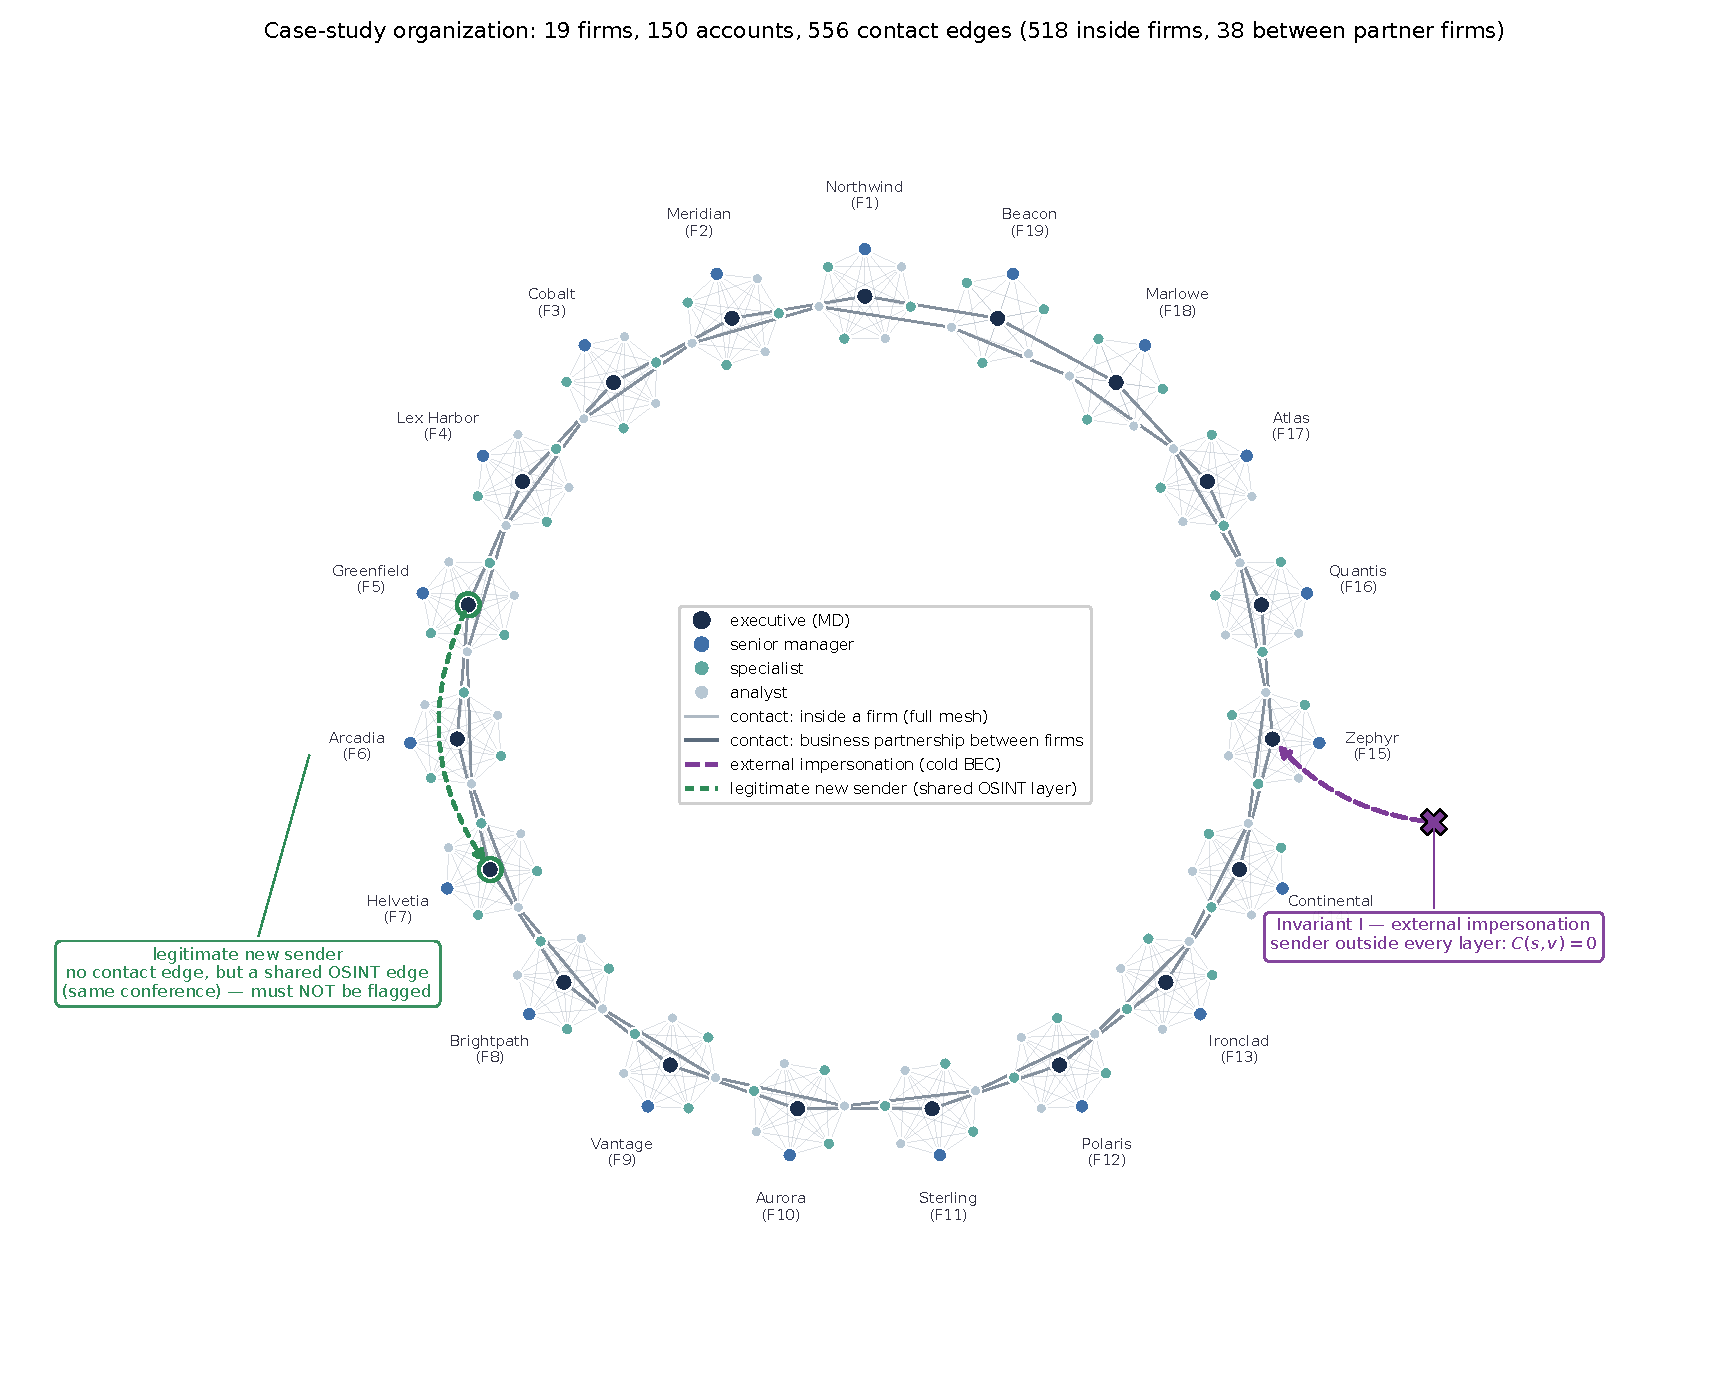
\includegraphics[width=0.95\textwidth]{fig_org_case_study_inv1.pdf}
\caption{Organizacja studyjna z danych populacji: $19$ firm na
pierścieniu partnerstw, $150$ kont kolorowanych po starszeństwie,
warstwa kontaktów ($556$ krawędzi). Nałożone dwa przypadki, które
detektor musi rozdzielić: impersonacja zewnętrzna spoza każdej
warstwy ($C(s,v){=}0$) oraz legalny nowy nadawca podłączony wyłącznie
przez współdzieloną warstwę OSINT (ta sama konferencja) --- który
nie może zostać oflagowany.}
\label{fig:m-casestudy}
\end{figure}

\begin{table}[htbp]\centering\small
\begin{tabular}{llcc}
\toprule
Warstwa & Krawędź (współdzielony fakt) & $w_L$ & \#krawędzi \\
\midrule
Kontakty       & nadawca pisał do odbiorcy        & $1{,}0$ & $556$ \\
Hierarchia     & ta sama firma                    & $0{,}9$ & $518$ \\
Domena         & ta sama domena pocztowa          & $0{,}8$ & $538$ \\
OSINT: konferencje & współdzielona konferencja    & $0{,}6$ & $167$ \\
OSINT: certyfikaty & współdzielony certyfikat     & $0{,}6$ & $389$ \\
OSINT: umiejętności & współdzielona umiejętność   & $0{,}5$ & $1144$ \\
OSINT: rutyna  & wsp. wzorzec komunikacji         & $0{,}4$ & $397$ \\
OSINT: wydarzenia & wsp. wydarzenie                & $0{,}4$ & $134$ \\
OSINT: platformy & wsp. platforma/handle           & $0{,}4$ & $534$ \\
OSINT: preteksty & wsp. wiarygodny pretekst        & $0{,}3$ & $159$ \\
OSINT: zainteresowania & pokrywające się zainteresowania & $0{,}3$ & $53$ \\
Czasowa        & ko-aktywność w tych samych godzinach & $0{,}5$ & $2528$ \\
\bottomrule
\end{tabular}
\caption{Warstwy multipleksu studyjnego: semantyka krawędzi, waga
ufności $w_L$ (równ.~\eqref{eq:m-coverage}), liczba krawędzi
(paczka reprodukcyjna, dane warstw).}
\label{tab:m-warstwy}
\end{table}

\section{Wyniki: niespójność międzywarstwowa jako mechanizm}
\label{sec:m-mechanizm}

Tabela~\ref{tab:m-inv1} testuje niezmiennik na dwóch przypadkach
z rysunku~\ref{fig:m-casestudy}. Fuzja warstw wiedzy domenowej
z rytmem podnosi AUC z $0{,}70$ (same kontakty) do $0{,}88$, podczas
gdy kontrola tasowania spada do losowego ($0{,}51$): przewaga
pochodzi ze struktury warstw i rytmu, nie z pojemności cech.
Najbardziej uderzająca jest strona fałszywych alarmów: detektor
kontaktowy flaguje \emph{każdego} legalnego nowego nadawcę
(FP $1{,}00$), multiplex --- \emph{żadnego} ($0{,}00$): pokrycie
OSINT ratuje legalnego nadawcę, który współdzieli z ofiarą
obserwowalny fakt.

Stwierdzamy jedną cyrkularność jawnie. W modelu zdarzeń legalny
nowy nadawca jest \emph{zdefiniowany} jako konto siedzące na
jakiejś warstwie OSINT ofiary, więc część likwidacji fałszywych
alarmów jest prawdziwa z konstrukcji: detektor kontaktowy nie może
tej warstwy zobaczyć, multiplex może. Netautologiczna jest reszta
dowodu: kontrola tasowania, która zachowuje brzegowe rozkłady cech
i spada do losowego ($0{,}51$, \emph{poniżej} samych kontaktów) ---
zysk zależy więc od rzeczywistej wspólnej struktury cech; sweep
fabrykacji, w którym fałszywe ślady erodują przewagę stopniowo,
nie skokowo (sekcja~\ref{sec:m-fabrykacja}); oraz wynik Enronu
(sekcja~\ref{sec:m-enron}), gdzie każda warstwa jest zbudowana
z prawdziwych nagłówków.

\begin{table}[htbp]\centering
\begin{tabular}{lcc}
\toprule
Model & AUC & FP na nowych nadawcach \\
\midrule
Kontakty               & $0{,}70$ & $1{,}00$ \\
Multiplex + rytm       & $\mathbf{0{,}88}$ & $\mathbf{0{,}00$} \\
Multiplex (tasowany)   & $0{,}51$ & --- \\
\bottomrule
\end{tabular}
\caption{Niespójność międzywarstwowa na grafie studyjnym (20 ziaren;
\texttt{exp\_multiplex.csv}: konfiguracja domyślna). Fuzja warstw
z rytmem podnosi AUC z $0{,}697$ do $0{,}875$ i likwiduje każdy
fałszywy alarm na legalnych nowych nadawcach; kontrola tasowania
spada do $0{,}505$.}
\label{tab:m-inv1}
\end{table}

Sygnał to zwięzła \emph{spójność}, nie pojemność: cztery jawne
miary spójności (pokrycie OSINT; znany nadawca poza rytmem; nowy
nadawca na OSINT; całkowicie poza grafem) dorównują pełnej
konkatenacji per-warstwa (\texttt{exp\_consistency.csv}: modele
liniowe $0{,}860$ wobec $0{,}840$; drzewa $0{,}860$ wobec $0{,}858$),
a ich wartość leży w wyjaśnialności i wdrożeniu single-query,
nie w czułości (recall).

\paragraph{Ablacja: co niesie sygnał.}
Rysunek~\ref{fig:m-ablation} pokazuje, skąd sygnał pochodzi --- i to
jest uczciwy rdzeń sprawdzania mechanizmu. Każda warstwa OSINT
dokłada marże (kontakty $0{,}57\to$ multiplex statyczny $0{,}66$),
ale cecha spójności czasowej dominuje: jej usunięcie cofa AUC
do $0{,}66$, dodanie --- prowadzi do $0{,}86$
(\texttt{exp\_ablation.csv}). Analiza per zagrożenie
(\texttt{exp\_layer\_by\_threat.csv};
rysunek~\ref{fig:m-bythreat}) potwierdza rozdział ról: dla nowych
nadawców sygnał niesie OSINT (sam OSINT $0{,}77$, sam czas $0{,}50$),
dla przejęć --- odwrotnie (sam czas $0{,}87$, sam OSINT $0{,}50$):
każda rodzina warstw jest krytyczna dla własnego trybu awarii.
Razem z tc-split (sekcja~\ref{sec:m-osint}) oznacza to, że większa
część zysku AUC pochodzi z kanału przejętych kont, gdzie rytm jest
rozstrzygający; dla impersonacji zewnętrznej zysk multipleksu
leży po stronie likwidacji fałszywych alarmów na legalnych nowych
nadawcach.

\begin{figure}[htbp]\centering
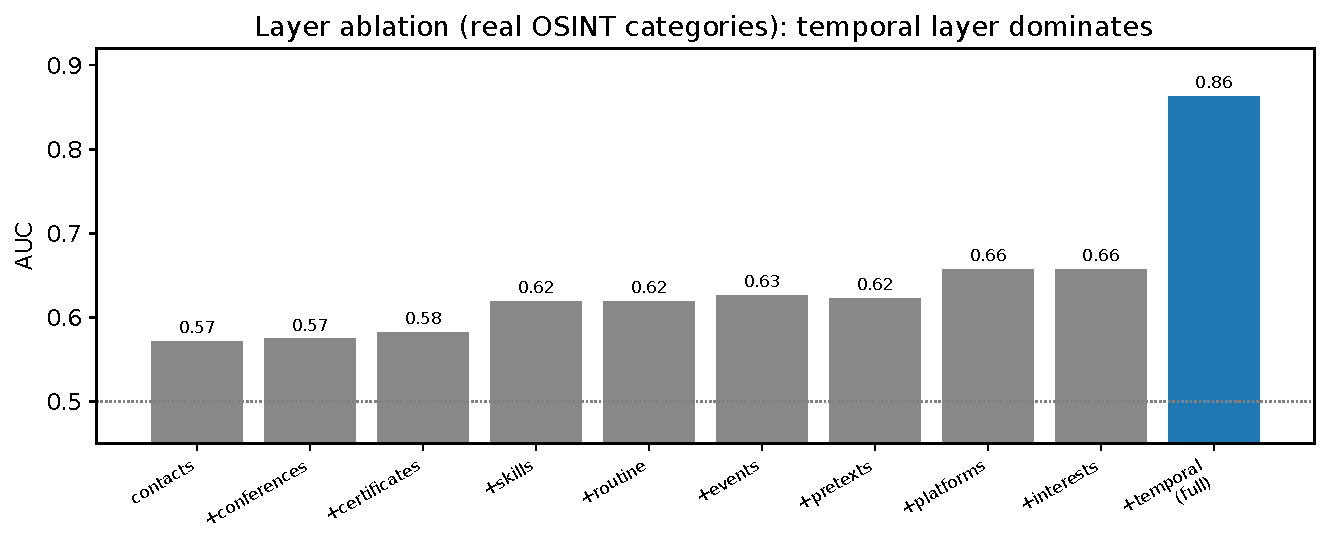
\includegraphics[width=0.9\textwidth]{fig_ablation.pdf}
\caption{Kumulatywna ablacja warstw (\texttt{exp\_ablation.csv}):
osiem warstw OSINT dokłada mało ponad kontakty ($0{,}57\to0{,}66$),
cecha spójności czasowej niesie resztę sygnału ($\to0{,}86$).}
\label{fig:m-ablation}
\end{figure}

\begin{figure}[htbp]\centering
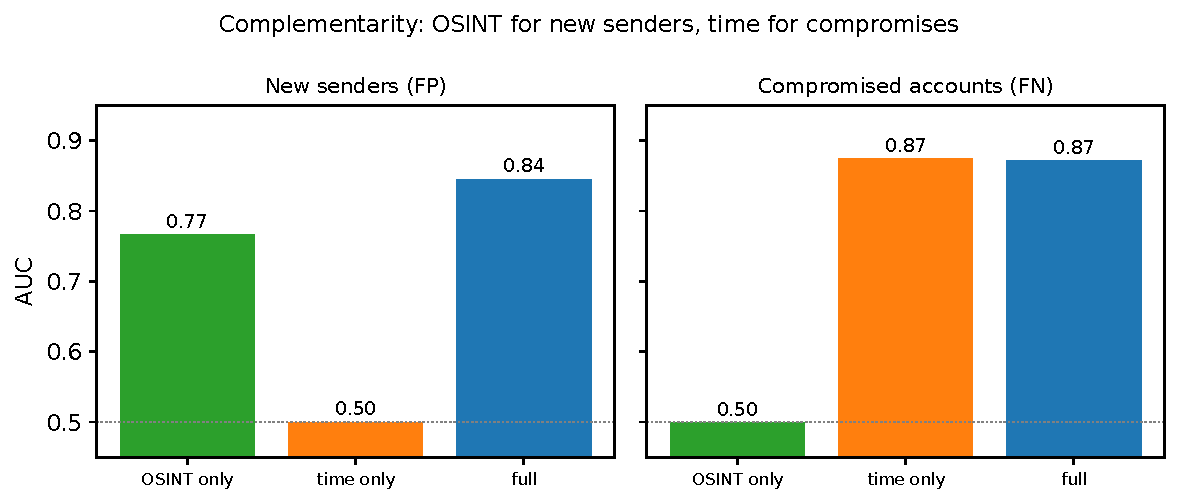
\includegraphics[width=0.9\textwidth]{fig_layer_by_threat.pdf}
\caption{Ablacja grupowa per zagrożenie: dla nowych nadawców
krytyczny jest OSINT, czas bezużyteczny; dla przejęć --- odwrotnie
(\texttt{exp\_layer\_by\_threat.csv}).}
\label{fig:m-bythreat}
\end{figure}

\section{Wyniki: uczciwa kontrola OSINT i tc-split}
\label{sec:m-osint}

Kontrola tasująca \emph{wszystkie} cechy nie izoluje wkładu samych
warstw OSINT; dlatego stosujemy kontrolę tasującą \emph{tylko}
warstwy OSINT (kontakty i rytm nietknięte) oraz nowy podział
\emph{tc-split}, który lokalizuje margines OSINT na plasterkach
konsystencji czasowej. Wyniki (\texttt{exp\_osint\_shuffle.csv},
\texttt{exp\_tc\_split.csv}):

\begin{itemize}
\item pełny multipleks $0{,}857$ [CI $0{,}852$--$0{,}863$]; bez OSINT
(kontakty+rytm) $0{,}826$; z tasowanym OSINT $0{,}821$; z tasowanym
wszystkim $0{,}503$. Wniosek: zysk niosą kontakty i rytm, a OSINT
dokłada $\sim\!0{,}03$ AUC --- i tasowanie tylko OSINT ten margines
zabiera;
\item na plasterku \emph{znany nadawca} multipleks nic nie zmienia
($0{,}79\approx0{,}79$); na plasterku \emph{w rytmie} (atak
w mimikrii) $0{,}58\to0{,}64$; na plasterku \emph{nowy nadawca}
$0{,}81\to0{,}90$ (czułość@1\% $0{,}11$) --- a tasowanie OSINT
cofa oba plasterki, więc jest to przyczynowy wkład OSINT;
\item wartość metody leży jednak po stronie fałszywych alarmów:
detekcja zimnej impersonacji pozostaje słaba (czułość $0{,}04$
przy FPR~1\%); OSINT służy do \emph{unieważniania} legalnych
nowych nadawców, nie do wykrywania podszywek.
\end{itemize}

\section{Wyniki: dekorelacja topologii}
\label{sec:m-topologia}

Prawie-tożsamość warstw strukturalnych
(kontakty$\approx$hierarchia$\approx$domena, Jaccard $\ge0{,}9$)
jest artefaktem generatora, który przypisuje jedną domenę na firmę.
Pokrętło dekorelacji $\rho$ przestraja kontakty między firmami
(\texttt{exp\_topology\_correlation.csv}): przy $\rho=0{,}8$
Jaccard spada do $0{,}39$, a niezależny wkład warstw strukturalnych
rośnie z $0{,}02$ do $0{,}25$ AUC --- znalezisko „efektywnie 3--4
niezależne warstwy" jest więc własnością zwartej populacji, nie
metody multipleks.

\section{Wyniki: realistyczna fabrykacja śladów}
\label{sec:m-fabrykacja}

Atakujący może sfabrykować ślad OSINT. Stwierdzenie~\ref{prop:fab}
przewiduje: przy fabrykacji i.i.d.\ z rozkładu \emph{prawdziwych}
śladów cechy istnienia tracą moc, kontrola permutacji ofiar jest
odporna na tempo fabrykacji, a zostają tylko cechy \emph{spójności}.
Pomiar (\texttt{exp\_multiplex.csv}, sweep fabrykacji;
tab.~\ref{tab:m-fab}): AUC multipleksu eroduje stopniowo
$0{,}88\to0{,}84$ ($10\%$ fałszywych krawędzi) $\to0{,}79$
($25\%$) $\to0{,}70$ przy $50\%$ --- poziomu samych kontaktów ---
z częściowym odbiciem $0{,}81$ przy $100\%$, gdy każdy atak niesie
ślad wyglądający na prawdziwy i rozdzielają już tylko rezydualne
sprzężenia; fałszywe alarmy na nowych nadawcach wracają od
$25\%$ fabrykacji. Kontrola tasowania pozostaje płaska
$0{,}50\pm0{,}01$ w całym zakresie --- zgodnie z częścią (ii)
stwierdzenia. Dla kontrastu, fabrykator \emph{legacy} (dowolna
warstwa, honorowana per zdarzenie) podnosi kontrolę tasowania
z tempem fabrykacji ($0{,}50\to0{,}60$ przy $50\%$;
\texttt{exp\_sweep\_fab.csv}) --- artefakt naruszenia (ii).

\begin{table}[htbp]\centering
\begin{tabular}{lcccccc}
\toprule
Fabrykacja OSINT & $0\%$ & $10\%$ & $25\%$ & $50\%$ & $75\%$ & $100\%$ \\
\midrule
AUC multipleksu   & $0{,}88$ & $0{,}84$ & $0{,}79$ & $0{,}70$ & $0{,}73$ & $0{,}81$ \\
Kontrola tasowania & $0{,}51$ & $0{,}50$ & $0{,}50$ & $0{,}50$ & $0{,}50$ & $0{,}50$ \\
\bottomrule
\end{tabular}
\caption{Realistyczna fabrykacja śladów (20 ziaren;
\texttt{exp\_multiplex.csv}): marża eroduje stopniowo do poziomu
samych kontaktów przy $50\%$ z częściowym odbiciem przy $100\%$,
zgodnie ze stw.~\ref{prop:fab}(i)+(iii); kontrola tasowania płaska
--- część (ii).}
\label{tab:m-fab}
\end{table}

\section{Wyniki: realny Enron i pułapka wycieku rytmu}
\label{sec:m-enron}

Z nagłówków korpusu Enron \citep{klimt2004enron} budujemy
\emph{realny} multipleks strukturalno-czasowy na $818$ nadawcach
i $\sim\!170$k zdarzeń: kontakty, współodbiorcy (konta adresowane
razem), ta sama domena pocztowa oraz rytm nadawcy --- wszystko
z samych nagłówków, \emph{bez} warstw OSINT (świadomy podział,
który trzyma wynik realny wolnym od syntetycznych nakładek).
Rytm estymujemy na dwa sposoby: z \emph{pełnej} historii --- co
wycieka okres ewaluacji do estymatu (cecha nieprzyczynowa,
def.~\ref{def:causal-feature}) --- albo z \emph{wczesnych} $60\%$
okresu z ewaluacją na późniejszych $40\%$ (uczciwy podział
czasowy); audyt off-hours wprawia frakcję legalnej poczty poza
estymowanym rytmem.

Tabela~\ref{tab:m-enronsplit} jest wynikiem metodologicznym
rozdziału. Pod wyciekającą estymacją samej warstwy czasowej,
detektor rytmu raportuje pozorną czułość $0{,}73$@FPR$1\%$;
pod uczciwym podziałem czasowym --- \emph{$0{,}00$ nawet przy
FPR~$5\%$}, bo ponad $5\%$ legalnej poczty wypada poza uczciwie
policzonym rytmem (próg nie spełnia FPR$\le1\%$ i czułość
jednobitowej cechy spada skokowo do zera, choć AUC jest wciąż
$0{,}75$). Pełny multipleks zachowuje czułość $0{,}14$
(AUC $0{,}82$), a z ruchem off-hours --- $0{,}01$--$0{,}15$
(AUC $0{,}77$): warstwy strukturalne liczone z wczesnych $60\%$,
jak rytm. Zgodnie z twierdzeniem~\ref{thm:lookahead} luka
$(0{,}73\to0{,}00)$ jest dokładnie obciążeniem look-ahead:
estymacja rytmu nadawcy na okresie ewaluacji daje pozorną
czułość, która znika pod kontrolą przyczynowości. To ostrzeżenie
dla całej klasy detektorów behawioralnych: \emph{każdy} rytm,
profil aktywności czy baseline liczony na pełnej historii zawyża
czujność detektora, który potem jest na nim ewaluowany.

\begin{table}[htbp]\centering
\begin{tabular}{lcccc}
\toprule
& \multicolumn{2}{c}{warstwa czasowa} & \multicolumn{2}{c}{pełny multipleks} \\
\cmidrule(lr){2-3}\cmidrule(lr){4-5}
Rytm estymowany z & AUC & cz.@1\% & AUC & cz.@1\% \\
\midrule
pełnej historii (\emph{z wyciekiem})   & $0{,}86$ & $0{,}73$ & $0{,}94$ & $0{,}88$ \\
wczesnego okna (\emph{podział czasowy}) & $0{,}75$ & $0{,}00$ & $0{,}82$ & $0{,}14$ \\
wczesnego okna $+$ off-hours (\emph{oba}) & $0{,}68$ & $0{,}00$ & $0{,}77$ & $0{,}01$ \\
\bottomrule
\end{tabular}
\caption{Kontrola wycieku rytmu na realnym grafie Enron (20 ziaren;
\texttt{exp\_enron\_temporal\_split.csv}): estymacja rytmu na pełnej
historii zawyża warstwę czasową do pozornej czułości $0{,}73$;
uczciwy podział czasowy sprowadza ją do $0{,}00$, podczas gdy pełny
multipleks trzyma $0{,}14$ (bez off-hours).}
\label{tab:m-enronsplit}
\end{table}

\begin{figure}[htbp]\centering
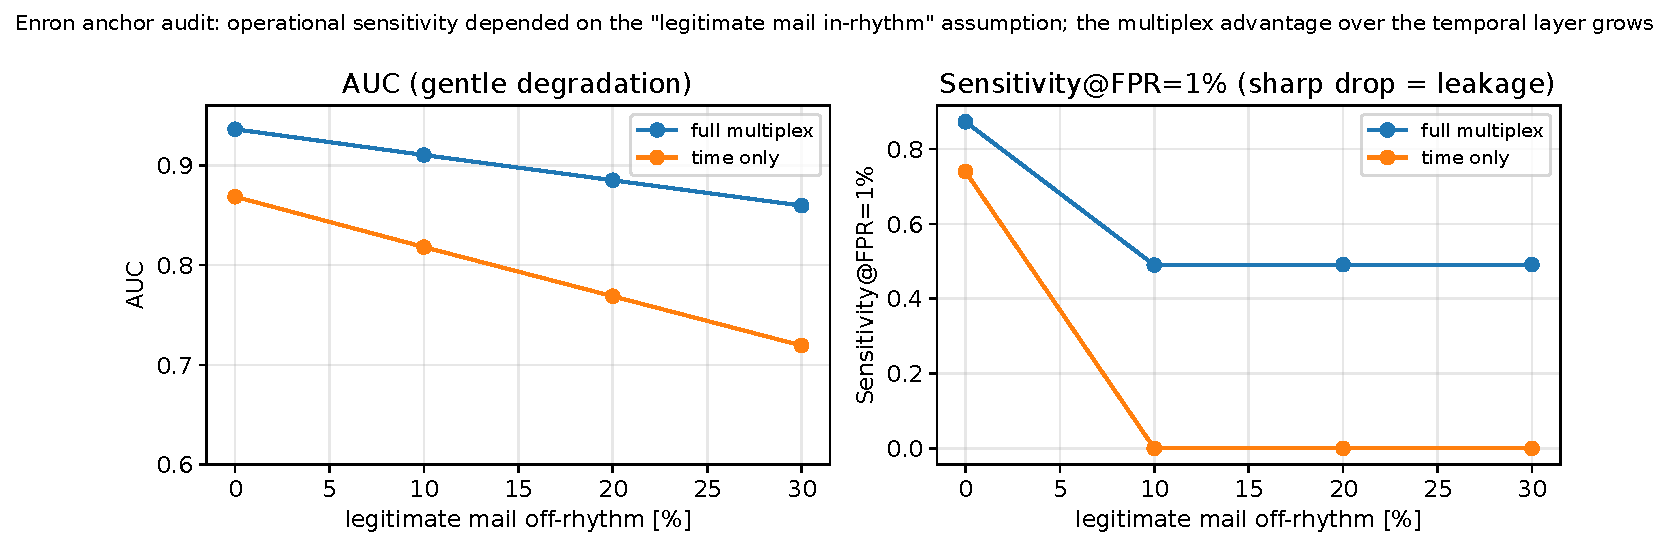
\includegraphics[width=0.9\textwidth]{fig_enron_audit.pdf}
\caption{Audyt Enron: AUC degraduje łagodnie z frakcją ruchu
poza godzinami pracy, ale operacyjna czułość@FPR$1\%$ warstwy
czasowej bez podziału czasowego była zawyżona --- po usunięciu
wycieku spada do zera, a przewaga multipleksu rośnie z frakcją
off-hours (paczka reprodukcyjna).}
\label{fig:m-enronaudit}
\end{figure}

\section{Wyniki: narażenie detektorowo-relatywne}
\label{sec:m-susc}

Tabela~\ref{tab:m-susc} rozkłada chybienia detektora fuzji
(czułość@FPR$1\%$, 20 ziaren, bootstrapowe 95\% CI) per kanał
ataku i starszeństwo ofiar. \emph{Kanał, nie ranga, napędza
narażenie}: zimna impersonacja zewnętrzna zostawia strukturalną
podłogę $\mathrm{Susc}\approx0{,}96$ na \emph{każdym} poziomie ---
bo żadna warstwa nie pokrywa nadawcy spoza grafu; przejęte konto
jest mniej groźne ($0{,}855$), bo znany kontakt poza rytmem to
ostre, nisko-FP sprzężenie. W kanale lateral obserwujemy ---
ale nie ogłaszamy jako odkrycia --- porządek odwrotny wobec
intuicji, że bogatsze osadzenie w grafie chroni: executive,
najbogatsi w warstwach wiedzy domenowej, są \emph{najbardziej}
narażeni ($\mathrm{Susc}=0{,}924$), juniorzy i mid-level
najmniej ($0{,}840$/$0{,}838$). Plauzybilne wyjaśnienie: bogato
osadzona ofiara ma dużo legalnej poczty poza rytmem i dużo
kontaktów międzywarstwowych, co poszerza przestrzeń, w której
atak wygląda na spójny. Powód ostrożności jest konstrukcyjny:
generator wiąże bogactwo warstw ze starszeństwem, więc kierunek
porządku części wynika z tego sprzężenia i wymaga testu pod
alternatywnymi przypisami. Tym, co twarde, jest: kanał dominuje
rangę, a starszeństwo nie kupuje ochrony.

\begin{table}[htbp]\centering\small
\begin{tabular}{llcc}
\toprule
Wymiar & Grupa & cz.@1\% & $\mathrm{Susc}$ \\
\midrule
\multirow{2}{*}{Kanał}
 & Impersonacja zewn. (zimne BEC) & $0{,}038$ & $\mathbf{0{,}962}$ \\
 & Przejęte konto (lateral)       & $0{,}145$ & $0{,}855$ \\
\midrule
\multirow{4}{*}{Starszeństwo (lateral)}
 & Executive & $\mathbf{0{,}076}$ & $\mathbf{0{,}924}$ \\
 & Senior    & $0{,}135$ & $0{,}865$ \\
 & Mid-level & $0{,}162$ & $0{,}838$ \\
 & Junior    & $0{,}160$ & $0{,}840$ \\
\midrule
\multirow{4}{*}{Starszeństwo (zimne BEC)}
 & Executive & $0{,}038$ & $0{,}962$ \\
 & Senior    & $0{,}040$ & $0{,}960$ \\
 & Mid-level & $0{,}042$ & $0{,}958$ \\
 & Junior    & $0{,}035$ & $0{,}965$ \\
\bottomrule
\end{tabular}
\caption{Narażenie detektorowo-relatywne detektora fuzji
(\texttt{exp\_susceptibility.csv}; 20 ziaren, FPR $=1\%$; 95\%
bootstrap CI po ziarnach --- patrz CSV): kanał ataku, nie ranga
ofiar, napędza narażenie; zimna impersonacja zostawia podłogę
$\approx0{,}96$ na każdym stanowisku.}
\label{tab:m-susc}
\end{table}

\section{Wyniki: granica graf--treść}
\label{sec:m-tresc}

Bo niezmiennik jest ślepy na zimną impersonację spoza grafu,
przypadek ten jest domeną treści. Eksperyment fuzji
(\texttt{exp\_content\_fusion.csv}; tab.~\ref{tab:m-tresc}) w dwóch
reżimach: w reżimie \emph{tell-tale} (atak z błędem treściowym)
treść (TF-IDF) rozdziela niemal idealnie ($0{,}997$) i multipleks
jest zbędny; w reżimie \emph{mimikrii} (BEC) treść jest ślepa
($0{,}496$), a sygnał niesie multipleks ($0{,}859$). Fuzja trzyma
się blisko lepszej modalności w każdym reżimie ($0{,}998$,
odpowiednio $0{,}851$) --- potwierdza, że treść i graf zawodzą
na \emph{różnych} atakach i że ich fuzja kosztuje mało; argument
za systemem hybrydowym. Jako sanity-check: na tym małym grafie
pojedynczy niestrojony multiplex GNN nie przewyższa jawnych cech
ręcznych (AUC $0{,}78$ wobec $0{,}86$ dla gradient boostingu) ---
w tej skali jawnie zdefiniowane cechy przynależności już łapią
sygnał.

\begin{table}[htbp]\centering
\begin{tabular}{lccc}
\toprule
Reżim & Treść & Multipleks & Fuzja \\
\midrule
Tell-tale (ślad w treści) & $0{,}997$ & $0{,}859$ & $\mathbf{0{,}998}$ \\
Mimikria (BEC)            & $0{,}496$ & $\mathbf{0{,}859}$ & $0{,}851$ \\
\bottomrule
\end{tabular}
\caption{Fuzja treści (TF-IDF) z multiplexem (AUC, 20 ziaren;
\texttt{exp\_content\_fusion.csv}): treść i graf zawodzą na
różnych atakach; fuzja trzyma się blisko lepszego w każdym
reżimie.}
\label{tab:m-tresc}
\end{table}

\section{Graf wiedzy domenowej jako narzędzie i cel}
\label{sec:m-kg}

Formalizm z sekcji~\ref{sec:m-model} nie jest li tylko aparatem
detekcji --- jego obiekt, graf wiedzy, jest coraz popularniejszym
\emph{narzędziem} do zapisywania wiedzy, w tym notatek. Ta sekcja
krótko sytuuje rozdział w tym kontekście i pokazuje, że jego
wyniki czytają się tam jako: mapa dla atakującego, cel ataku
i zasada detekcji anomalii.

\paragraph{Grafy wiedzy jako narzędzie.} Grafy wiedzy są
dojrzałym paradygmatem reprezentacji wiedzy \citep{hogan2021knowledge,
ji2022survey}: od otwartych grafów encyklopedycznych po
organizacyjne grafy wiedzy i tematyczne --- w tym grafy wiedzy
o zagrożeniach (CTI) budowane wspomaganie modelami językowymi
\citep{fieblinger2024actionable,cheng2024ctinexus}. W warstwie
osobistej i zespołowej grafowa struktura notatek stała się
standardem narzędzi typu \emph{second brain} (Obsidian, Logseq,
Roam): notatka jest węzłem, a konspektyczny link --- krawędzią;
w efekcie graf NOTATEK organizacji jest często cichym, bogatym
\emph{shadow} tego samego grafu wiedzy domenowej, który
aksjomatyzujemy w definicji~\ref{def:m-dkg}. Trzeci nurt ---
fuzja z modelami językowymi: grafy wiedzy osadzone w
architekturach GraphRAG i pamięci agentów jako warstwa
wierzygodnego kontekstu \citep{pan2024roadmap,edge2024graphrag}
--- czyni z grafu wiedzy nie tylko nośnik notatek, ale czynnik
\emph{decyzyjny}: odpowiedź systemu jest tak dobra, jak
wierzygodność krawędzi, z których ją zretrievowano.

\paragraph{Ta sama struktura jest mapą dla atakującego.}
Wszystko, co w grafie wiedzy organizacji jest pomocne --- kim
jest dany pracownik, z kim pracuje, o czym pisze, w jakim rytmie
--- jest też dokładnie materiałem OSINT, z którego atakujący
buduje pretekst (sekcja~\ref{sec:p-osint}; \citealp{edwards2017panning,
brown2025web}). Graf publikowany, udostępniany na zewnątrz
albo rekonstruowalny ze śladów (konferencje, certyfikaty,
profile) jest \emph{mapą ataku}: personalizacja, która kiedyś
wymagała wiedzy eksperckiej, sprowadza się do zapytań po
grafie. Model zagrożeń tego rozdziału bierze to explicite:
atakujący zna warstwy i może w nie celować.

\paragraph{Jest też celem ataku.} Gdy graf wiedzy zasila detekcję
lub GraphRAG, kontrola nad krawędziami jest kontrolą nad
decyzją. Wektorami są: (i)~\emph{fabrykacja krawędzi} --- dodanie
do publicznego śladu faktów łączących atakującego z ofiarą,
podnoszenie spójności międzywarstwowej; twierdzenie
\ref{prop:fab} i sweep z sekcji~\ref{sec:m-fabrykacja} pokazują
właśnie ten mechanizm: do $\sim\!50\%$ fałszywych krawędzi
marża detektora eroduje do poziomu samych kontaktów, a przy
pełnej fabrykacji każdy atak niesie ślad nierozróżnialny
od prawdziwego; (ii)~\emph{trucie korpusu i osadzeń} ---
literatura ataków adversarialnych na grafy pokazuje, że
dodanie kilku starannie dobranych krawędzi zmienia klasyfikację
GNN \citep{zugner2018adversarial,zugner2019adversarial,
dai2022towards}; jeśli obrona działa na grafie, który atakujący
może wzbogacić, nieprzyczynowe cechy (def.~\ref{def:causal-feature})
i kontrola tasowania (stw.~\ref{prop:shuffle}) są warunkiem
oznaczenia ataku, nie opcją; (iii)~\emph{iniekcja treści} ---
w architekturach RAG dokument wciągnięty do korpusu staje się
przyszłą „wiedzą", którą system przywoła jako kontekst;
zatruty dokument to odpowiednik sfałszowanej notatki
w grafie wiedzy.

\paragraph{Zasada detekcji anomalii uogólnia się.} Niezmiennik
rozdziału --- prawdziwa relacja jest spójna w wielu warstwach
naraz --- jest w istocie ogólną zasadą detekcji anomalii
na grafach wiedzy i notatkach: encja, notatka lub krawędź,
która pojawia się w jednej warstwie i jest przeczona przez
pozostałe (kontakty, hierarchia, rytm, treść notatek), jest
sygnałem anomalii --- tak detekują oszustwa metody
niespójności między perspektywami \citep{liu2020alleviating},
a szersza rodzina nienadzorowanych detektorów anomalii
grafowych \citep{akoglu2015graph,liu2021anomaly,li2025umgad,
behrouz2022anomaly} czyta ten sam wzorzec. Praktyczna reguła
dla narzędzi notatek i CTI-graphów brzmi więc tak, jak brzmi
protokół rozprawy: (a)~warstwa za warstwą, z jawną wagą ufności
$w_L$ i rytem $\tau$; (b)~ocena spójności wielowarstwowej zamiast
pojedynczych flag; (c)~każda cecha i każdy baseline liczony
wyłącznie z przeszłości (tw.~\ref{thm:lookahead}); (d)~kontrola
fabrykacji sprawdzająca, ile fałszywych krawędzi eroduje marżę
(stw.~\ref{prop:fab}). Z oddali: wandalizm --- celowe wstawianie
fałszywych tez --- jest operacyjną rzeczywistością publicznych
grafów wiedzy, z własnym torem detekcji
\citep{heindorf2017wsdmcup,sarabadani2017tools,heindorf2019debiasing}
i korpusami historii rewizji \citep{schmelzeisen2022wikidated};
trucie grafów GraphRAG (recepta PoisonedRAG przeniesiona na
konstrukcję grafu) pokazuje, że „kilka słów zniekształca graf"
\citep{wen2025fewwords,kepo2026,zou2024poisonedrag}, a wstrzyknięcie
pośrednie pozwala odzyskanemu zatrutemu dokumentowi stać się
instrukcją dla modelu \citep{greshake2023not}.

\paragraph{Trzy pomiary artykułu C.} Ten obraz jest mierzalny w paczce
reprodukcyjnej (artykuł C; \texttt{exp\_fab\_edge\_detection.csv},
\texttt{exp\_rag\_poison.csv}, \texttt{exp\_kg\_poisoning.csv}):
(i)~przy fabrykacji i.i.d.\ z rozkładu łącznego prawdziwych śladów
detekcja \emph{krawędziowa} jest bezradna --- cechy istnienia AUC
$\approx0{,}50$, kontrola permutacji $0{,}50$, a pozorny sygnał
spójności ($0{,}56$--$0{,}65$) jest artefaktem definicji
prawdziwości, który rozprawa ujawnia jawnie (empiryczna granica
stw.~\ref{prop:fab}(i)--(iii)); (ii)~w retrieval GraphRAG-lite atak
zoptymalizowany pod zapytanie (recepta PoisonedRAG) korumpuje $100\%$
top-5 ofiar, a bramka spójności (wsparcie w warstwach wewnętrznych
LUB $\ge2$ niezależne ślady OSINT) zeruje go --- podnosząc koszt
atakującego z jednego wstrzykniętego tekstu do $\ge2$ niezależnych
sfałszowanych publicznych śladów na ofiarę, przy cenie $92{,}5\%$
oflagowanych legalnych międzyorganizacyjnych jedno-faktowych
więzi na czystym korpusie; (iii)~na publicznym FB15k-237 spójność
relacyjna ranguje sfabrykowane trójki na AUC $0{,}72$ (cechy
istnienia $0{,}52$; kontrast sparowany Wilcoxon $p{=}0{,}005$,
$\delta{=}1{,}0$), ale sens@FPR$1\%\approx0$ --- podłoga
izolowanych trójek prawdziwych czyni z niej narzędzie triażu,
nie filtr progowy, zgodnie z regułą bazy rozdziału formalnego;
a fabrykator \emph{path-preserving}, który zna cechę wspólnych
sąsiadów i kopiuje mierzoną przez nią własność, neutralizuje ją
(AUC $0{,}71\to0{,}56$) --- wyścig zbrojeń jest cecha po cecha,
przetrwać może tylko potwierdzenie przez własności, które
atakujący musi skopiować łącznie.

\section{Podsumowanie rozdziału}
\label{sec:m-podsumowanie}

\paragraph{RQ3 (sygnał międzywarstwowy).} Niespójność międzywarstwowa
jest rzeczywistym sygnałem na grafie studyjnym: fuzja warstw z rytmem
podnosi AUC $0{,}70\to0{,}88$ i likwiduje $100\%$ fałszywych alarmów
na legalnych nowych nadawcach, kontrola tasowania spada do losowego
($0{,}51$), a uczciwa kontrola tylko-OSINT i tc-split lokalizują
margines OSINT ($+0{,}03$ AUC globalnie; $0{,}81\to0{,}90$ na
plasterku nowych nadawców; zysk z tasowania OSINT znika). Uczciwe
znalezisko: cecha spójności czasowej niesie większość sygnału
rankingowego, warstwy strukturalne są na zwartej populacji prawie
współliniowe (Jaccard $0{,}93$; po dekorelacji $\to0{,}39$ ich
niezależny wkład rośnie do $0{,}25$). Wartość praktyczna metody
leży po stronie fałszywych alarmów, nie czujności na podszywki
(zimna impersonacja: $0{,}04$@1\%).

\paragraph{RQ4 (narażenie i granice).} Miara narażenia
detektorowo-relatywnego pokazuje, że narażenie napędza kanał ataku,
nie ranga ofiar (zimna impersonacja: podłoga $\approx0{,}96$ na
każdym stanowisku; w kanale lateral executive najbardziej narażeni
--- $0{,}924$ --- a bogactwo osadzenia nie kupuje ochrony);
treść i graf zawodzą na różnych atakach i ich fuzja jest blisko
lepszego z nich w każdym reżimie. Granice ewaluacji tej klasy
detektorów ujawnia pułapka wycieku rytmu: pozorna czujność
$0{,}73$@1\% detektora rytmu estymowanego na pełnej historii
spada do $0{,}00$ pod uczciwym podziałem czasowym, podczas gdy
multipleks trzyma $0{,}14$ --- empiryczna instancja
twierdzenia~\ref{thm:lookahead} i praktyczna reguła: rytm, profil
i baseline behawioralny estymować wyłącznie z okresu
\emph{poprzedzającego} ewaluację.
